
\documentclass{jcgt}
\usepackage{subfigure}

\setciteauthor{Richard J. Arietta}
\setcitetitle{CUDA Simulation and Rendering of Voxelized Cloud Volumes on the GPU}

% Mark submissions with the date of submission using the following line:
%\submitted{\today}

% Once an article is accepted accepted, switch to the following line and comment the preceding one. The editor will supply the argument values.
\accepted{July 4, 2013}{July 4, 2013}{July 4, 2013}{Editor Name}{2}{1}{1}{1}{2013}
\seturl{http://jcgt.org/published/0002/02/01/}




%%%%%%%%%%%%%%%%%%%%%%%%%%%%%%%%%%%%%%%%%%%%%%%%%%%%


\begin{document}

\title{CUDA Simulation and Rendering of Voxelized Cloud Volumes on the GPU}

\author
       {Richard J. Arietta\\University of Pennsylania}

% Optional teaser image
\teaser{
  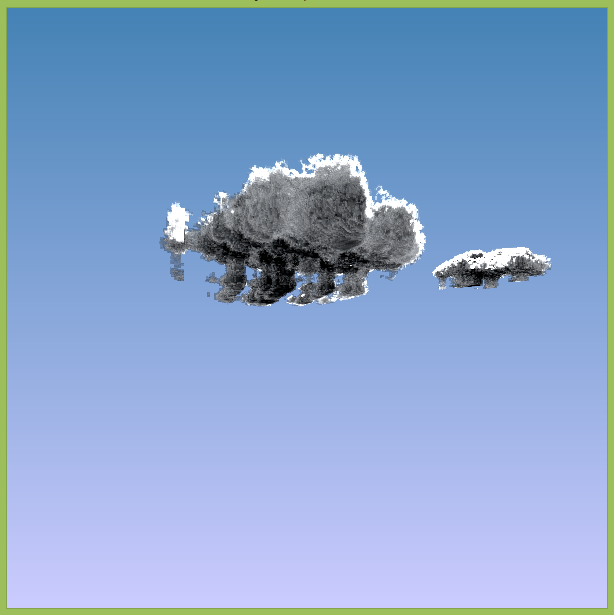
\includegraphics[width=1.5in]{images/cloudDaytime.png}
  \label{fig:teaser}
  \caption{An example of voxelized cloud volumes rendered
  		   with this program.}
}


\maketitle
\thispagestyle{firstpagestyle}

\begin{abstract}
\small
For my final project, I have implemented a program to create voxelized cloud 
volumes, simulate their growth and dynamics over time, and render them effectively 
to produce a final image/video sequence. All simulation and rendering computation 
is done entirely on the GPU using CUDA and C++ programming languages. This paper 
will go into the details of each step involved in creating the final rendered 
sequences, as well as exploring some of the final results, analyzing performance, 
and discussing the scope of the work and its future.

\end{abstract}


%-------------------------------------------------------------------------
\section{Introduction}
\label{sec:introduction}
Voxelized volume structures are useful in graphics applications
for representing changing and/or transmissive particle bodies. As opposed to
hollow meshes or implicit surfaces, voxelized volumes are geometry that has 
been subdivided into a 3D grid of cubic elements -- or "voxels" -- that 
each represent a particle within the body. Because of this approach, 
volumetric rendering of voxel systems allows us to render bodies with density and 
color information throughout the interior rather than just on exterior surfaces.

Thus, voxelized volumetrics prove to be an effective way to render
atmospheric clouds. Clouds are made up of particles, each of which can be defined
by a voxel, and each of these particles has partial opacity depending on
the geometry of the cloud at any given time. These particles 
interact with light such that the most dense regions will transmit the least light,
while the less dense regions will transmit much more light, leading to partial 
transparency and limited self-shadowing.

I have implemented a program to create and render these clouds, as well as simulate 
their growth and motion in a believable way. All simulation and rendering is 
implemented on the GPU in CUDA.

\subsection{Relevant Related Work}
\label{sec:relatedwork}

Much work has been done on this subject by others. One crucial piece of related 
work that I adapted comes from the book Game Engine Gems 2. I utilized Kane's 
approach to cloud growth in my simulations.

\section{Process}
The process of creating dynamic cloud volumes can be broken down into 3 stages: 
Initialization and Storage of Cloud Volume Data Structures; Simulation Computations
for Cloud Growth, Expiration, and Animation; and Rendering using Ray Marching Techniques. 
The first stage is responsible for establishing the cloud volume data structures. The second 
involves modifying and storing these data structures at each time-step of the simulation. 
The last involves determining the visible volumes given a virtual camera and computing 
luminance values to produce a final image. Each stage will now be explored in detail.

\subsection{Initialization and Storage of Cloud Volume Data Structures}
In order to generate volumetric clouds, I first need to establish a data type for storing
them. My cloud scenes were organized as follows:

\begin{itemize}
\item Each cloud in the scene was represented by its own "volume" struct. A volume struct
	  contains: the size of a voxel; the number of voxels along each axis of the volume's 
	  bounding box; the step size to be taken when marching a ray through the volume 
	  (see the section on rendering); the material; etc. Most importantly, each volume 
	  contains an array of "voxel" structs representing the particle grid.
\item Each "voxel" struct contains: a density used for light transmission calculations; a
	  probability for each of three simulation values (extinction, vapor, and
	  phaseTransition, each of which describe how likely a particle is to attain or lose
	  its cloud status); and a char representing the state of the voxel at the current
	  time step.  
\end{itemize}

\noindent
When the program is first called, each of the voxels' fields is initialized according to
a noise function. I have implemented a Perlin noise generation function in
3D space, limiting the size and shape of the noise to a hemi-ellipsoid bounding volume.
All voxels outside a certain radius from the volume's center, or below
a certain height representing the base of the cloud. are given a density of
zero, and their state is set to reflect that they do not carry a cloud particle. Within
the bounding region, each voxel is assigned a density corresponding to its Perlin noise 
function value in 3D space, scaled by its distance from the local origin. This ensures 
that the center of the cloud is the densest and the outer layers of the cloud are 
transmissive. The same scaling is applied to the simulation probabilities (see next 
section). The voxels nearest the center of the base are more likely accumulate vapor
or shift phase and less likely to lose cloud status at any given frame, and vice versa. 
At initialization, only the voxels at the base of the vloud are marked as clouds. The cloud
will grow up from this base layer. These values are stored out into the array of volumes 
to be used in simulation.

\subsection{Simulation Computations for Cloud Growth, Expiration, and Animation}

The technique used for simulation of cloud growth/dynamics is based on a
chapter on cloud rendering in Game Engine Gems 2, contributed by Frank Kane. The idea
behind the simulation is that each voxel contains a state with three bits: one bit
for if the voxel is currently a cloud particle; one bit for if the 
voxel contains water vapor; and one bit for if the voxel is ready for a phase
transition from water vapor to liquid cloud particle. As indicated previously,
these values are all set during initialization, leaving only the lowest cloud level
as cloud particles. Much like real cumulus clouds, I want the to grow up from the
base into a noisy form. Therefore, for each simulation step, we \texttt{OR} the state
of a particle with its neighbors in the horizontal plane and its neighbor below. Using
this new \"phaseBit\" and a series of 3 random numbers compared to the voxel's
probabilities, we determine at each time step whether the state of the voxel changes.
If the conditions are met to satisfy either probability, then the voxel will either
accumulate or lose vapor, phase transition readiness, or cloud form. 

In addition to this simulation, the clouds were each given a specified velocity so
that the whole volume would translate horizontally with time.

\subsection{Rendering using Ray Marching Techniques}

After performing each simulation, the cloud volumes are rendered. I accomplish
this task with a ray marching algorithm. Casting rays from the camera (as in path tracing),
I look for intersections with a volume's bounding box. When a volume is intersected, I 
step through the volume and integrate the opacity and color values of each voxel until 
a threshold is reached. The step size $s$ along the ray is determined by the volume. 
Therefore, for each initial intersection point $\bar{x}$ and ray direction $\hat{n}$, 
we initialize the transmittance value $T$ to $1.0$ and the color value $C$ to black. 
At each new step point inside the volume, luminance and opacity are accumulated according
to these equations:

\begin{align}
\label{raymarch}
x_i & += \hat{n} \Delta s\\
\label{deltaT}
\Delta T & =  \exp(-\kappa \Delta s \rho(x_i))\\
\label{trans}
T & *= \Delta T \\
\label{color}
C & += \frac{1-\Delta T}{-\kappa}(\bar{c}(x_i)\odot \bar{F})TQ(x_c,\hat{n},\Delta s_i, x_l)
\end{align}

\noindent
where $\kappa$ is a predefined attenuation for density, $(\bar{c}(x_i)\odot \bar{F})$
is the product of the light color and the material color, and $Q(x_c,\hat{n},\Delta s_i, x_l)$
is the lighting value accumulated by tracing along a secondary ray from the voxel in
question to the light source. These values are accumulated up to a certain predefined threshold. 
Then the RGB value is blended with the existing value at that pixel
according to its transparency.

\section{Results}

While this suimulation is not accurate in terms of cloud dynamics as dictated by physics, 
it provides a realistic growth and change of cloud volumes at a much cheaper cost. 
The results can be seen in Figure~\ref{fig:cloud_renders}. The rendering provides believable interplay
between the light source and the cloud particles. Note the silver lining present around the
top edges of the clouds, and the self-shadowing from the particles in the densest regions.


\begin{figure}[htb]
  \centering
  \hfill
  \subfigure[TitleA]{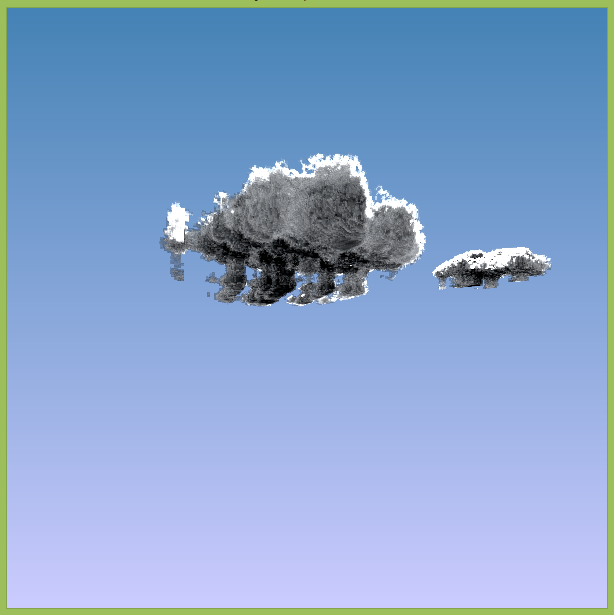
\includegraphics[width=0.35\columnwidth]{images/cloudDaytime.png}}
  \hfill
  \subfigure[TitleB]{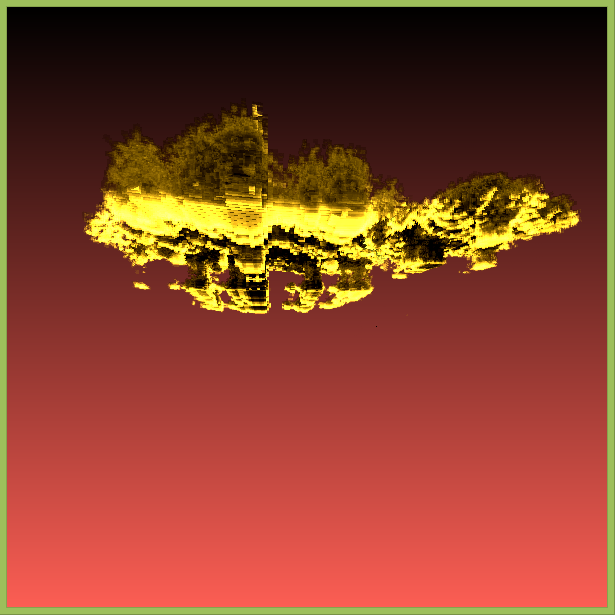
\includegraphics[width=0.35\columnwidth]{images/cloudSunset.png}}
  \hfill
  \caption{\label{fig:cloud_renders}
     These are two different cloud images saved out from the simulations. The one on the
     left is meant to resemble daytime clouds, while the one on the right is meant to
     simulate the light effects on a cloud body during sunset hours.}
\end{figure}

\section{Analysis}

This analysis focuses on runtime frames per second and performance speed. This is something
I tried hard to optimize, but was unable to get the simulation/rendering to run in perfect
real time. However, they do perform at a highly interactive rate and I do not think the
end product suffers greatly.

As you can see in Figure~\ref{fig:performance_distribution}, most of the processing at runtime
is evenly split between simulation and rendering. Memory management pays a small role in the
FPS, while initialization is only run once and is therefore minimal.

\begin{figure}[htb]
  \centering
   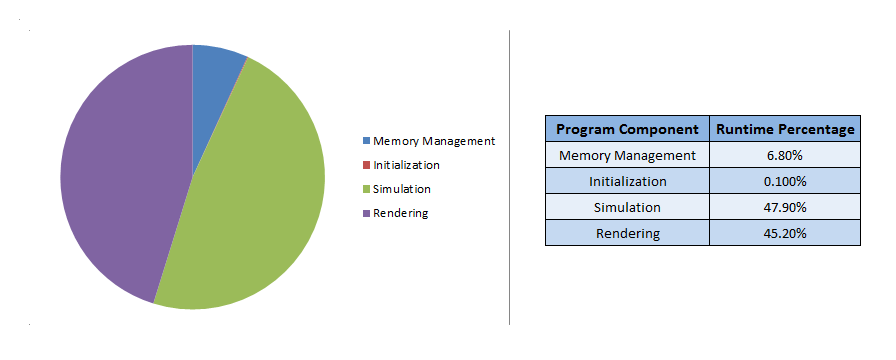
\includegraphics[width=0.7\columnwidth]{images/Performance.png}
   \caption{\label{fig:performance_distribution}
     These are the percentages of runtime computation. As you can see, most of the processing
     is performed in simulation and rendering steps, which is to be expected.}
\end{figure}

Furthermore, the use of a threshold cutoff while tracing rays through the volume seems
to have had a positive impact on runtime. Figure~\ref{fig:threshold_performance} shows
all the rays in which this threshold was crossed for transparency along camera rays
for a given scene and the included increase in FPS during runtime. This cutoff was also
implemented along secondary light rays.

\begin{figure}[htb]
  \centering
  \hfill
  \subfigure[TitleA]{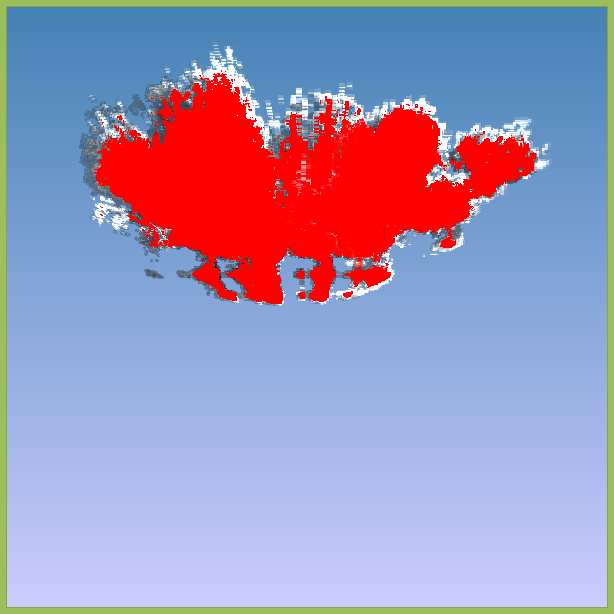
\includegraphics[width=0.4\columnwidth]{images/threshold.png}}
  \hfill
  \subfigure[TitleB]{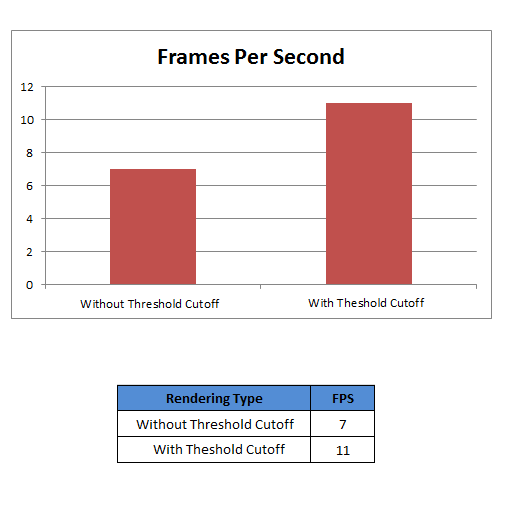
\includegraphics[width=0.4\columnwidth]{images/thresholdperf.png}}
  \hfill
  \caption{\label{fig:threshold_performance}
     This image illustrates the role of threshold cutoff during rendering. Each pixel
     in red corresponds to a ray that was terminated before exiting the volume because
     the transparency had already fell below this threshold. Utilizing this method
     increased runtime on this example scene by 36\%, from 7 FPS to 11 FPS.}
\end{figure}

\section{Discussion}

Moving forward with this project, there are several things I would like to address. First,
when I set out to complete the project, I had hoped to provide some kind of user interface
for creating the cloud volumes with proxy geometry and certain user defined settings.
Unfortunately I did not get to this. I think that this would be an important addition, 
since these animations are artistic in nature and providing user control would only make them more relevant.

Additionally, I would like to improve the renderer by incorporating a weighted sampling aspect
for the voxel grid to achieve a less voxelized appearance for the clouds without having to
greatly increase the number of voxels.

\section*{Author Contact Information}

\hspace{-2mm}\begin{tabular}{p{0.5\textwidth}p{0.5\textwidth}}
Richard J. Arietta \newline
University of Pennsylvania \newline
\href{mailto:rarietta@seas.upenn.edu}{rarietta@seas.upenn.edu}

\end{tabular}

\small
\afterdoc

\end{document}
